\section{Models}

The model architecture is adapted from the functional design of SAM,
and also informed by the development of OPUS and UrbanSim. The
functionality in SAM focuses on the allocation of land use by
sector to grid cells, from aggregate information at a mid-level
geography such as RAZs or MPAs.  By reference to the UrbanSim model system,
this functionality is approximately equivalent in purpose to the
real estate development model component of UrbanSim, with some key
differences.  UrbanSim attempts to include a complete representation
of the real estate market, with occupants (consumers: households
and jobs), buildings and land (suppliers: developers and property
owners), and prices (markets: hedonic regressions representing the
interaction of suppliers and consumers).

The architecture for the model system proposed for AZ-SMART is based
on a 3-year plan, and incorporates the complete market
representation as in UrbanSim, and a multi-level geography and model
system.  We describe this in the Full Model System subsection below,
and then focus on a Phase 1 Model System in the subsequent section.

\subsection{Full Model System}
The full model system proposed for AZ-SMART involves some
hybridization and extension of elements of UrbanSim and SAM-IM.
Below we itemize the core elements of the full model system
architecture.  These are depicted in Figure \ref{figFlow}, which
shows the model components, their sequence of operation, and the
data objects on which the models operate.  Note that the data are
hierarchically organized in the center of the figure, with
aggregation relationships moving from bottom to top.


\begin{figure}[h]
\begin{center}
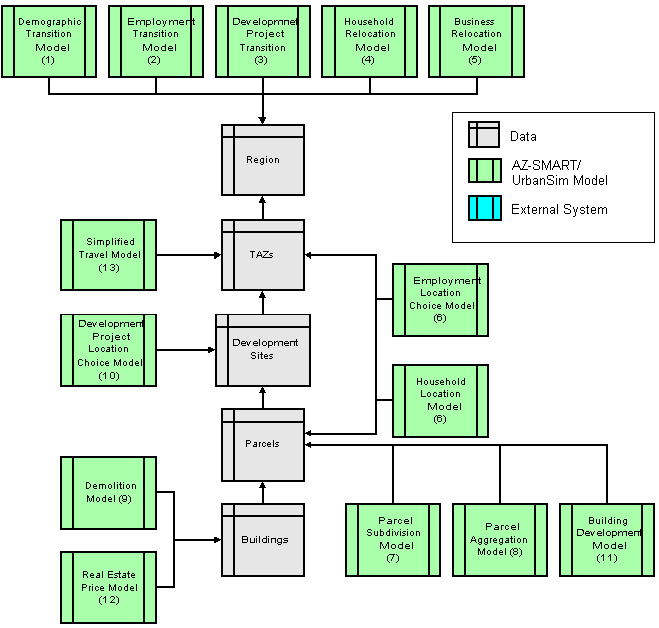
\includegraphics[scale=0.8]{figures/flow.png}
\caption{AZ-SMART Full Model Architecture} \label{figFlow}
\end{center}
\end{figure}

\begin{itemize}

\item \emph{Land-Structure-Occupant Accounting}: The full market
representation and explicit representation of and accounting of
Land-building-occupant objects and their relationship is proposed
for the full model architecture.

\item \emph{Parcels and Buildings}: Land could be represented by
parcels, land use polygons, or cells, but it is expected that
the parcel concept would be used as the principal representation
of land, and that in areas that do not have parcel data available,
land use polygons could be used in a way that treats them as
equivalent to (possibly large) parcels.  Note that there are many
to one relationships from buildings to land and from occupants to
building.  That is, a building may contain multiple occupants,
and a parcel (or land use polygon) may contain multiple buildings.
In the event that building data is not available, it could be
imputed, to preserve a consistent data model.

\item \emph{Development Projects, Sites and Templates}: Development 
 projects include both
 known \emph{development projects} which the user wishes to
 incorporate into the simulation, and also development projects
 predicted by the simulation and assigned to \emph{development
 sites}.  For predicted development projects, a set of pre-defined
  \emph{development templates} provide a set of configurations of
  development that include at a minimum the mix of building types
  (land uses), density, size and timetable for development.

\item \emph{Multi-level Model}: The full model system would use
a multi-level approach, incorporating parcels as the lowest level
(buildings are linked to parcels), and for the forseeable future,
one higher level geography to represent an intermediate geography
between the county and the parcel.  Traffic Analysis Zones (TAZ)
are proposed as the basis for this mid-level geography in the full
 model, simplifying the interface with the travel model system.
 There are behavioral and practical reasons for using a two-level
 geography in the model system.  Behaviorally, it is based on the
 expectation that consumers looking for a location (e.g. a household
  searching for a house) compare neighborhoods, and select properties
  to examine based on their assessment of the neighborhoods. In
  practical terms, the two-level geography provides a more convenient
  way to interface models in a modular way, for example to interface
  the travel model system, or to run the model system for corridor or
  area studies where more detail is needed in a subset of the planning
  region and less is needed outside of this focus area.

\item \emph{Microsimulation}: The proposed architecture is based on
explicit representation of the agents and objects being modeled at a
microscopic level.  Parcels, buildings, businesses (or jobs),
households, and eventually, persons (for supporting activity-based
travel models and workplace choice models and individual-level
accessibility calculations).

\item \emph{Temporal Dynamics}: The model system would be able to
use a specified time interval, such as 5-year or 1-year steps,
between which it would simulate changes to the state of each object
and agent in the system (construction of new buildings or conversion
of existing ones, movement of households and businesses from one
location to another, creation of new households or businesses).

\item \emph{Models and Interface}: A set of models will be interfaced
through a common data store, and managed by a Model Coordinator that
controls their execution and implements events (changes to the data)
proposed by models.  The individual models would be the following:

\begin{itemize}
\item Demographic Transition (Region): Reconciles the control totals
of population (by household type) with the database - adding households
to the database or removing them if a household type is declining.
\item Employment Transition (Region): Reconciles the control totals
of employment (by sector) with the database - adding businesses (jobs)
to the database or removing them if a sector is declining.
\item Household Relocation (Region): Predicts whether a household will
move from their existing residence during the next time step.
\item Business Relocation (Region): Predicts whether a business  (job)
will move from their existing location during the next time step.
\item Household Location (TAZ and Parcel): Predicts the building that
a new or moving household will choose from among the set of buildings
with a vacanct unit.
\item Business Location (TAZ and Parcel): Predicts the building that a
new or moving business (job) will choose from among the set of buildings
with sufficient vacanct space.
\item Parcel Subdivision (Parcel): Predicts the number and size of
parcels to create from a large parcel that is to be subdivided to create
a development project. Depending on whether the project is known or
predicted this will use information provided in the development project
description or drawn from a development template.
\item Parcel Aggregation (Parcel): Combines adjacent parcels to create
a \emph{development site} suitable to place a development project.
\item Development Project Proposal Choice Model (Parcel): Predicts the
parcel chosen to locate a development project.
\item Event Coordinator (Building): Generates building records from 
the known and simulated development projects, based on their Development
Velocity Functions, and adds them to the parcel the project is on.
\item Real Estate Price Model (Parcel): Predicts the price
per unit (or sqft) for each land use type at each location (parcel).
\item Simplified Travel Model (TAZ): An abbreviated travel model with
just a.m. peak, and other simplifications to provide a relatively
high-speed regional travel model to use in intermediate years preceding
the target year for the regional transportation plan.
\end{itemize}
\end{itemize}

The models proposed for implementation in Phase 1 of this project are
described in greater detail in the following section.

\subsection{Phase 1 Model System}
Phase 1 of the AZ-SMART project focuses on the allocation of totals
defined at the RAZ (or other) geographic level to parcels or land use
polygons.  

In the following
description of the model system architecture, we a design
option of using parcels or land use polygons.  For most purposes this would not affect
the formulation of the models.  We propose initially to implement the model using 
parcels, using data for PIMA and Maricopa Counties.

The following models are the focus of model development in Phase 1:

\begin{itemize}
\item Real Estate Price Model (Parcel)
\item Development Project Proposal Choice Model (Parcel)
\item Land Subdivision (Parcel)
\item Land Aggregation (Parcel)
\item Travel Model Interface (current emme/2 or new TransCad model)
\end{itemize}

The following models would be implemented for completeness, but would
use a simple specification.

For the sake of brevity, we will refer to parcels below, but please keep in mind
that this would initially be done with land use polygons, and that land use 
polygons would continue to be used in counties without parcel data.  Please refer
to figure \ref{figParcelDataModel} for details on the data model that these models 
would be operating on.

\begin{itemize}
\item Demographic Transition (RAZ)
\item Employment Transition (RAZ)
\item Development Project Transition (RAZ)
\item Household Location (Parcel)
\item Business Location (Parcel)
\end{itemize}

The following components of the full model system would be deferred until after Phase 1:

\begin{itemize}
\item Simplified Travel Model (TAZ)
\item Higher - level model to replace DRAM/EMPAL
\end{itemize}

The proposed model architecture has the following steps, using a 5-year time interval.

Each model is described in the sequence it would be run within a simulation period.

\subsubsection{Building Development Model}

 

\subsubsection{Demographic Transition Model}

The first task is to translate mid-level model predictions of population and employment by RAZ (or
other mid-level geography) into predicted demands for housing units and land area of non-residential
uses by type. The \emph{Demographic Transition Model} will compare the sum of the household
population to the control target for a specified year, and if the existing population is less than the control
total, it will add the needed number of households to the households table, without a location being specified.
If the current population of a particular type is greater than the control total target, the model will remove
households of this type randomly until the control total is met.


The Economic Transition Model does the same with employment, comparing the sum of employment by
industry sector (the sectors from Dram/Empal) to the employment control totals, and adds new jobs if the
existing employment is less than the control total for a sector.  If the existing employment is greater, it
removes jobs of this sector randomly from the jobs table until the control target it met.

\subsubsection{Determine Development from Scheduled (Active) Projects}

In this step, we compute the quantity of development expected in a RAZ (or other mid-level geography) for each land use
sector based on the velocity within Scheduled (Active) Development projects, and assigns the development generated
by Active Development Projects to the parcels (or polygons) within those developments.  These tasks are
handled by an \emph{Model Coordinator} that implements events that have been scheduled and applies
them to the database.  Scheduled Projects would be stored in the database, and the model coordinator
at the beginning of a simulation period would load any events that overlap this time frame.  For all scheduled
development projects (user specified projects, and also projects predicted by the model in a previous simulation
period), the model coordinator will look up the velocity function for the project, and add the predicted number
of buildings to the buildings dataset. 

\subsubsection{Generate Development Proposals}

The \emph{Development Project Proposal Choice Model} will begin by evaluating for each development site 
the applicable development constraints, and
generating a set of proposed development projects, from the set of development templates
that would fit on the site and are consistent with land use regulations.  
Note that more than one project that might be allowed on a site, and
there may be sites that would not allow any projects to be developed.  The result of this step
would be a list of proposed development projects, from which the most likely projects should be
selected, while imposing the constraint that once a project is selected for a site, the site is
excluded from further consideration for other projects, and that once the project committments
reach a stage that at completion they would cause the vacancy rate in a given property type (land
use) to exceed a long-term stable rate (a break-even rate for developers), a project will not be
accepted for development.  This is equivalent to the role of the financial sector providing
capital to developers for financing construction projects. When vacancy rates exceed a long-term
level that is seen as a high-risk threshold, the likelihood of being able to secure financing for
a development project should fall quickly.

\subsubsection{Development Scoring: Estimated Return on Investment}
The evaluation of which development proposals are most likely to be implemented requires
computing some kind of a scoring function, to use the term as applied in the SAM model.  In SAM,
each land use sector has its own scoring function, and the user specifies a pre-determined order
to apply the model to the set of land use sectors.  Since the scoring functions cannot be compared
across sectors, there is no way to decide which land use sector would outbid or out-compete for
a particular site.  We propose to improve on this approach by using a common scoring mechanism:
estimated return on investment.  This would allow comparisons to be made among all development
proposals, and economic logic to be more directly used in making the predictions of what kind of
development will occur at different locations.

As noted earlier, the proposed approach is consistent with a view of the decision-making agent as
a financial agent who is evaluating which development proposals to provide financing for.  The 
probability of being successful in securing financing is likely to be proportional
to the return on investment on a project.  Simply put, the ratio of the expected profit to the amount
invested is a reasonable measure of the relative
probability of one project being developed as compared to other potential projects.  Note that this
approach combines and reconciles the two contrasting approaches used in real estate economics and
finance: the site looking for a use (the landowner perspective) and the use looking for a site (the developer 
perspective).  If we generate possibly multiple project proposals on each development site,
and then compare their expected profit not only across proposals for the same site, but also across
sites, then we have an approach that accounts for the competition among developers for sites, and
among land owners for development.  Note that this is a significant advance over the current
specification of both UrbanSim and SAM-IM.

We can estimate the expected profit by a fairly straightforward method: hedonic regression.  This
approach is already well supported in OPUS and UrbanSim, and allows the specification and estimation
of models with price as the dependent variable (or log price), and a set of structural and locational
attributes on the right hand side of the model.  It essentially 'decomposes' the sales transaction
price (or assessed value if sales data are not readily available) into component marginal prices for
each attribute, such as bedrooms, square footage, age, accessibility and other locational
and structural characteristics.

\begin{equation}
ln(P) = \alpha + \beta X + \gamma Z
\end{equation}

where $ln(P)$ is the natural log of the price per unit for residential, and per square foot for nonresidential 
buildings and land; $X$ is a set of location characteristics, and $Z$ is a set of characteristics of the 
building.  Parameters $\beta$ and $\gamma$ would be estimated using Ordinary Least Squares, with OPUS
estimation utilities.  The particular variables to be used in the model specification can be determined
during the model development phase, through iterative testing of alternative specifications.  A relatively
simple model specification with good explanatory power is preferred over model complex specifications.

Using the Real Estate Price Models for each property type, we can estimate the resulting final value of any
development project by predicting the valuation of the component parts of a project and summing them
over the components.  If we subtract the value of the site prior to development, and subtract the
cost of the construction (and possibly the cost of demolishing existing buildings on the site), then
we have a working estimate of the expected return on investment from the development.

\begin{equation}
ROI^* = \frac{\sum{e^{ln(P^*)}Q^*}-\sum{e^{ln(P^0)}Q^0 - C_c - C_s - C_d - C_f}}{\sum{e^{ln(P^0)}Q^0 + C_c + C_s + C_d + C_f}}
\end{equation}

where $ROI^*$ is the estimated return on investment on a proposed project, $P^*$ is the estimated market value per unit (sqft)
of the building after completion, $Q^*$ is the quantity or size of the development project (number of units, number of square feet),
$P^0$ is the estimated pre-development value per unit of the existing property, and $Q^0$ is the pre-development quantity
of development.  $C_c$ is the construction cost of the development, $C_s$ is the cost of site preparation, including provision of 
infrastructure to the site, $C_d$ is the cost of demolition of any existing buildings on the site, and $C_f$ is the financing cost over
the duration of time that the project is under development and on the market. 

The costs in the model could initially be estimated using simple constants, but would be available for refinement using more
sophisticated estimation algorithms over time.

\subsubsection{Predict Development Project Proposal Probabilities}
Once the development project proposals have been evaluated and the expected 
return on investment from each has been
estimated, we can use a simple multinomial logit model to generate the probabilities of each being
developed.  The principle term in the utility function is the expected ROI, and the probability of
development will be proportional to the relative profit of the proposed project.

\begin{equation}
Pr(i) = \frac{e^{ROI_i}}{\sum_{j \in J}{e^{ROI_j}}}
\end{equation}

\subsubsection{Sample Development Projects Until Demand Met}
Once we have generated the probability distribution across projects, we may use that to sample from.
We draw samples from the probability distribution and add them to the list of committed projects,
at each step updating the amount of committed space by type, and evaluating whether we have reached
a cutoff threshold for any property types.  Once the committed projects reach a point that the next
project adds enought space to exceed the structural vacancy rate, then the algorithm will reject any
additional proposals that would further increase the vacancy rate in that property type.  The drawing
process proceeds until the threshold vacancy rate has beeen exceeded in all property types or a
predefined number of iterations has been reached.

\subsubsection{Iterate over RAZs (or other geography) and Allocate Unplaced Development Projects}

Once allocation of all development in a RAZ or other mid-level geography is completed, process the
next RAZ. If not all development could be allocated in a RAZ, accumulate unmet demand within a higher
level geography to be processed in a final iteration. If needed, allocate unmet demand from higher
level (MPA for example), to Development Sites as above.

\subsubsection{Data Implications}
The implications for data requirements of the proposed Phase 1 model design are intended to be relatively
modest, allowing the effort to focus on developing the software infrastructure for the AZ-SMART project.  However,
there are some new data requirements implied by the model design.  One of these is the development templates.
These templates can be drawn from information about the known developments, so may not involve any new
data collection effort, but rather just additional analyis of data that is already in hand.  Another data requirement
of the proposed approach is information on real estate values.  These could come from the county assessors
office, or from a real estate research source that records sales transactions.  An alternative to sales transactions 
is the use of assessed values, which are available for all properties, but may have some limitations depending on
how these assessments are made by the assessors' offices.

Parcel data may eventually be desirable to use, but initially, as noted earlier, we propose to rely principally on the
existing land use data used in SAM, to reduce the data preparation effort and focus more on functional model and
software development.

\subsection{Parcel Subdivision}
One of the new models that will be needed in Phase 1 is a parcel
subdivision model.  As an initial approach, we propose to avoid the
problem of operating on the topology of the parcel polygon, and
instead just create new parcel records that become children of the
original parcel, containing all the relevant attributes including
area, and respecting the total area of the original parcel, but not
being depicted by polygons.  This approach would manage risk and
avoid spending too much of the development effort on this one
aspect.  We can also explore options for algorithms to
cartographically subdivide parcels.

If this is not sufficiently detailed for MAG or PAG, then options for developing a topological subdivision of polygons
will be explored in greater depth, so that alternative approaches can be assessed for feasibility and level of effort.

\subsection{Parcel Aggregation}
A parcel aggregation model will also be needed in Phase 1.  We
propose to initially develop this model using user-specified
redevelopment area polygons, that can be treated as development
sites.  We will define the spatial relationship of parcels within
each redevelopment area to the development area polygon, and assign
the polygon to the set of development sites.  At this point, the
cost of development on one of these sites would include the cost of
acquiring the parcels contained in the site and demolishing any
existing development on them.  This will reduce their expected
profit as compared to greenfield development, but is economically
realistic.

In a later phase, we may be able to generate redevelopment districts
through an algorithm that finds parcels meeting certain conditions,
and then attempts to 'grow' the development site by finding
neighboring parcels that when combined, would generate a profitable
development site.  Our assessment is that this would be beyond the
scope of Phase 1, however.
